\section{Ejercicio 8}

Presentamos el siguiente lote corrido con distintos semillas de aleatoridad y tamaño de quantum.
El objetivo es mostrar que al ser pseudo-random, la semilla no produce favoritismo entre los procesos y que los diferentes quantum no van a alterar el fairness del algoritmo

*6 TaskBatch 20 5 \\

Hacer procesos largos iguales cortarlos antes de terminar y ver que el tiempo de CPU de cada uno tiende a igual, y que si veo màs que antes se mantiene, 
entonces da que es un scheduler "fairness"

Ver ejemplos de entrada salida y ver que estos tienden a tener mas CPU que los otros ya que la probabilidad aumenta por tener màs tickets\\

Semilla de Aleatoridad = 1 y Quantum = 3
\begin {center}
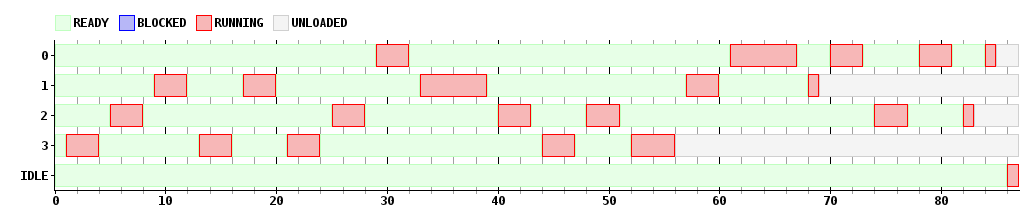
\includegraphics[width=16cm]{../simusched/outputs/ej8/sl-ej8-1-3.png}
\end {center}
Se puede ver en este ejemplo que si tomamos sectores de la corrida, vemos como la obtención de recursos se mantiene constante.\\
Tomemos los casos de 0 a 40 y de 40 a 80.
De 0 a 40: el primer: 4, el segundo: 6, el tercero: 4, el cuarto: 10, el quinto: 8, el sexto: 7 \\
De 40 a 80: el primer: 10, el segundo: 12, el tercero: 4, el cuarto: 0, el quinto: 10, el sexto: 0 \\
Si bien notamos concentraciones en la primera parte sobre los últimos procesos y en la segunda sobre los primeros podemos notar la uniformidad de los mismos (tomar en cuenta que es un algoritmo probabilístico).
Es decir el primero obtuvo 14, el segundo 18, el tercero 8, el cuarto 10, el quinto 18 y el sexto 7, y en un algoritmo fairness deberían haber obtenido 80/6 = 14 cada uno.
Por lo que podemos ver que la uniformidad se mantiene, lo que tiende a que terminen juntos como en el roundrobin tal como se ve en el gráfico.\\

Semilla de Aleatoridad = 5 y Quantum = 2
\begin {center}
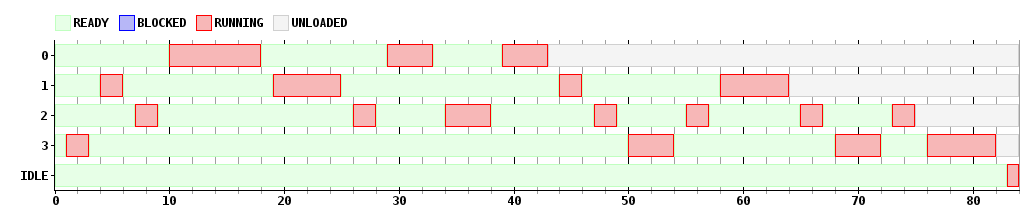
\includegraphics[width=16cm]{../simusched/outputs/ej8/sl-ej8-5-2.png}
\end {center}
Tomemos los casos de 0 a 40 y de 40 a 80.
De 0 a 40: el primer: 2, el segundo: 4, el tercero: 2, el cuarto: 12, el quinto: 2, el sexto: 11 \\
De 40 a 80: el primer: 10, el segundo: 6, el tercero: 4, el cuarto: 2, el quinto: 5, el sexto: 9 \\
En total: el primer: 12, el segundo: 10, el tercero: 6, el cuarto: 14, el quinto: 7, el sexto: 20 \\
Algoritmo Fairness = 14 cada uno.\\
De vuelta podemos notar como en promedio los procesos tienden a estar cerca del algoritmo fairness

Semilla de Aleatoridad = 3 y Quantum = 5
\begin {center}
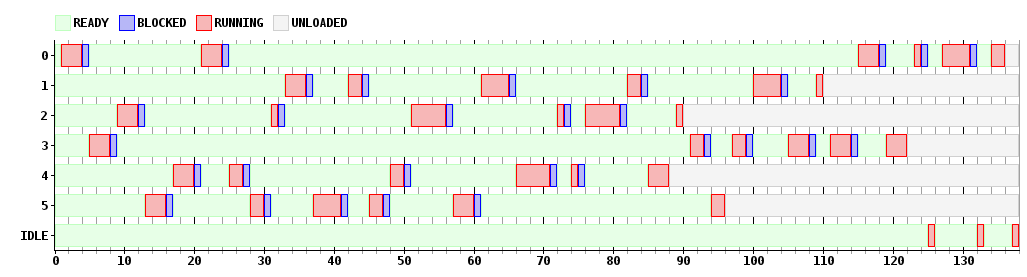
\includegraphics[width=16cm]{../simusched/outputs/ej8/sl-ej8-3-5.png}
\end {center}
Tomemos los casos de 0 a 40 y de 40 a 80.
De 0 a 40: el primer: 8, el segundo: 4, el tercero: 6, el cuarto: 4, el quinto: 6, el sexto: 10 \\
De 40 a 80: el primer: 0, el segundo: 8, el tercero: 12, el cuarto: 0, el quinto: 11, el sexto: 9 \\
En total: el primer: 8, el segundo: 12, el tercero: 18, el cuarto: 4, el quinto: 17, el sexto: 19 \\
Algoritmo Fairness = 14 cada uno.\\
En este caso no fue tan fairness como otros, pero es un buen ejemplo para probar que si bien tiende a ser fairness, no es detirminístico y no deja de ser probabilístico\\
Semilla de Aleatoridad = 2 y Quantum = 12
\begin {center}
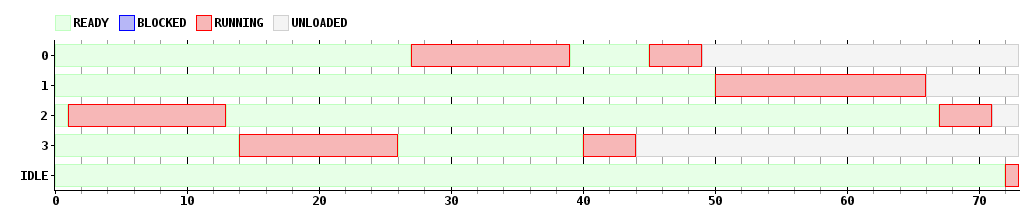
\includegraphics[width=16cm]{../simusched/outputs/ej8/sl-ej8-2-12.png}
\end {center}
Acá el proceso 5 ganó mucho la lotería porque la cantidad de tickets después de cada bloqueo es mucho mayor ya que es proporcional a la cantidad de tiempo que no usás y al ser un quantum grande, aquel que se bloquea gana muchos tickets para el próximo sorteo. Aquí se puede notar como la compensación de tickets varía según si los procesos se bloquean más que otros, y si el quantum es grande dándole más posiblidad de obtener más tickets.\\


En conclusión, el algoritmo tiende a ser fairness como RoundRobin o tantos otros. Esto va a depender de la configuración y mientras más sepamos de los procesos de entrada podemos acomodarlos a nuestra ventaja.
En caso de que elijamos quantum grandes, la compensación va a ser más grande en caso de un bloqueo ya que lo más probable es que haya gastado poco tiempo, por lo cual para el próximo sorteo en el que participe, va a tener
muchos más tickets que el resto teniendo así más probabilidad de ganar la lotería.
Es decir que correr el mismo proceso n veces la probabilidad de que gane, va a ser igual en cada uno de estos n experimentos
Debemos aclarar que si bien estámos hablando de un algoritmo random, computacionalmente es pseudo-random, es por eso que se probaron distintas semillas de aleatoridad y se ve claramente que no afecta al algortimo.
